\section{Deep Gated Network }
The deep gated network (DGN) set up was introduced by \cite{npk}. The DGN treats the gates as masks and decouples them from the weights. The DGN is a ``simple experimental" setup to characterise the role played by the gates in a `standalone' manner.  
\subsection{Setup}
\FloatBarrier
\begin{figure}[H]
\begin{center}
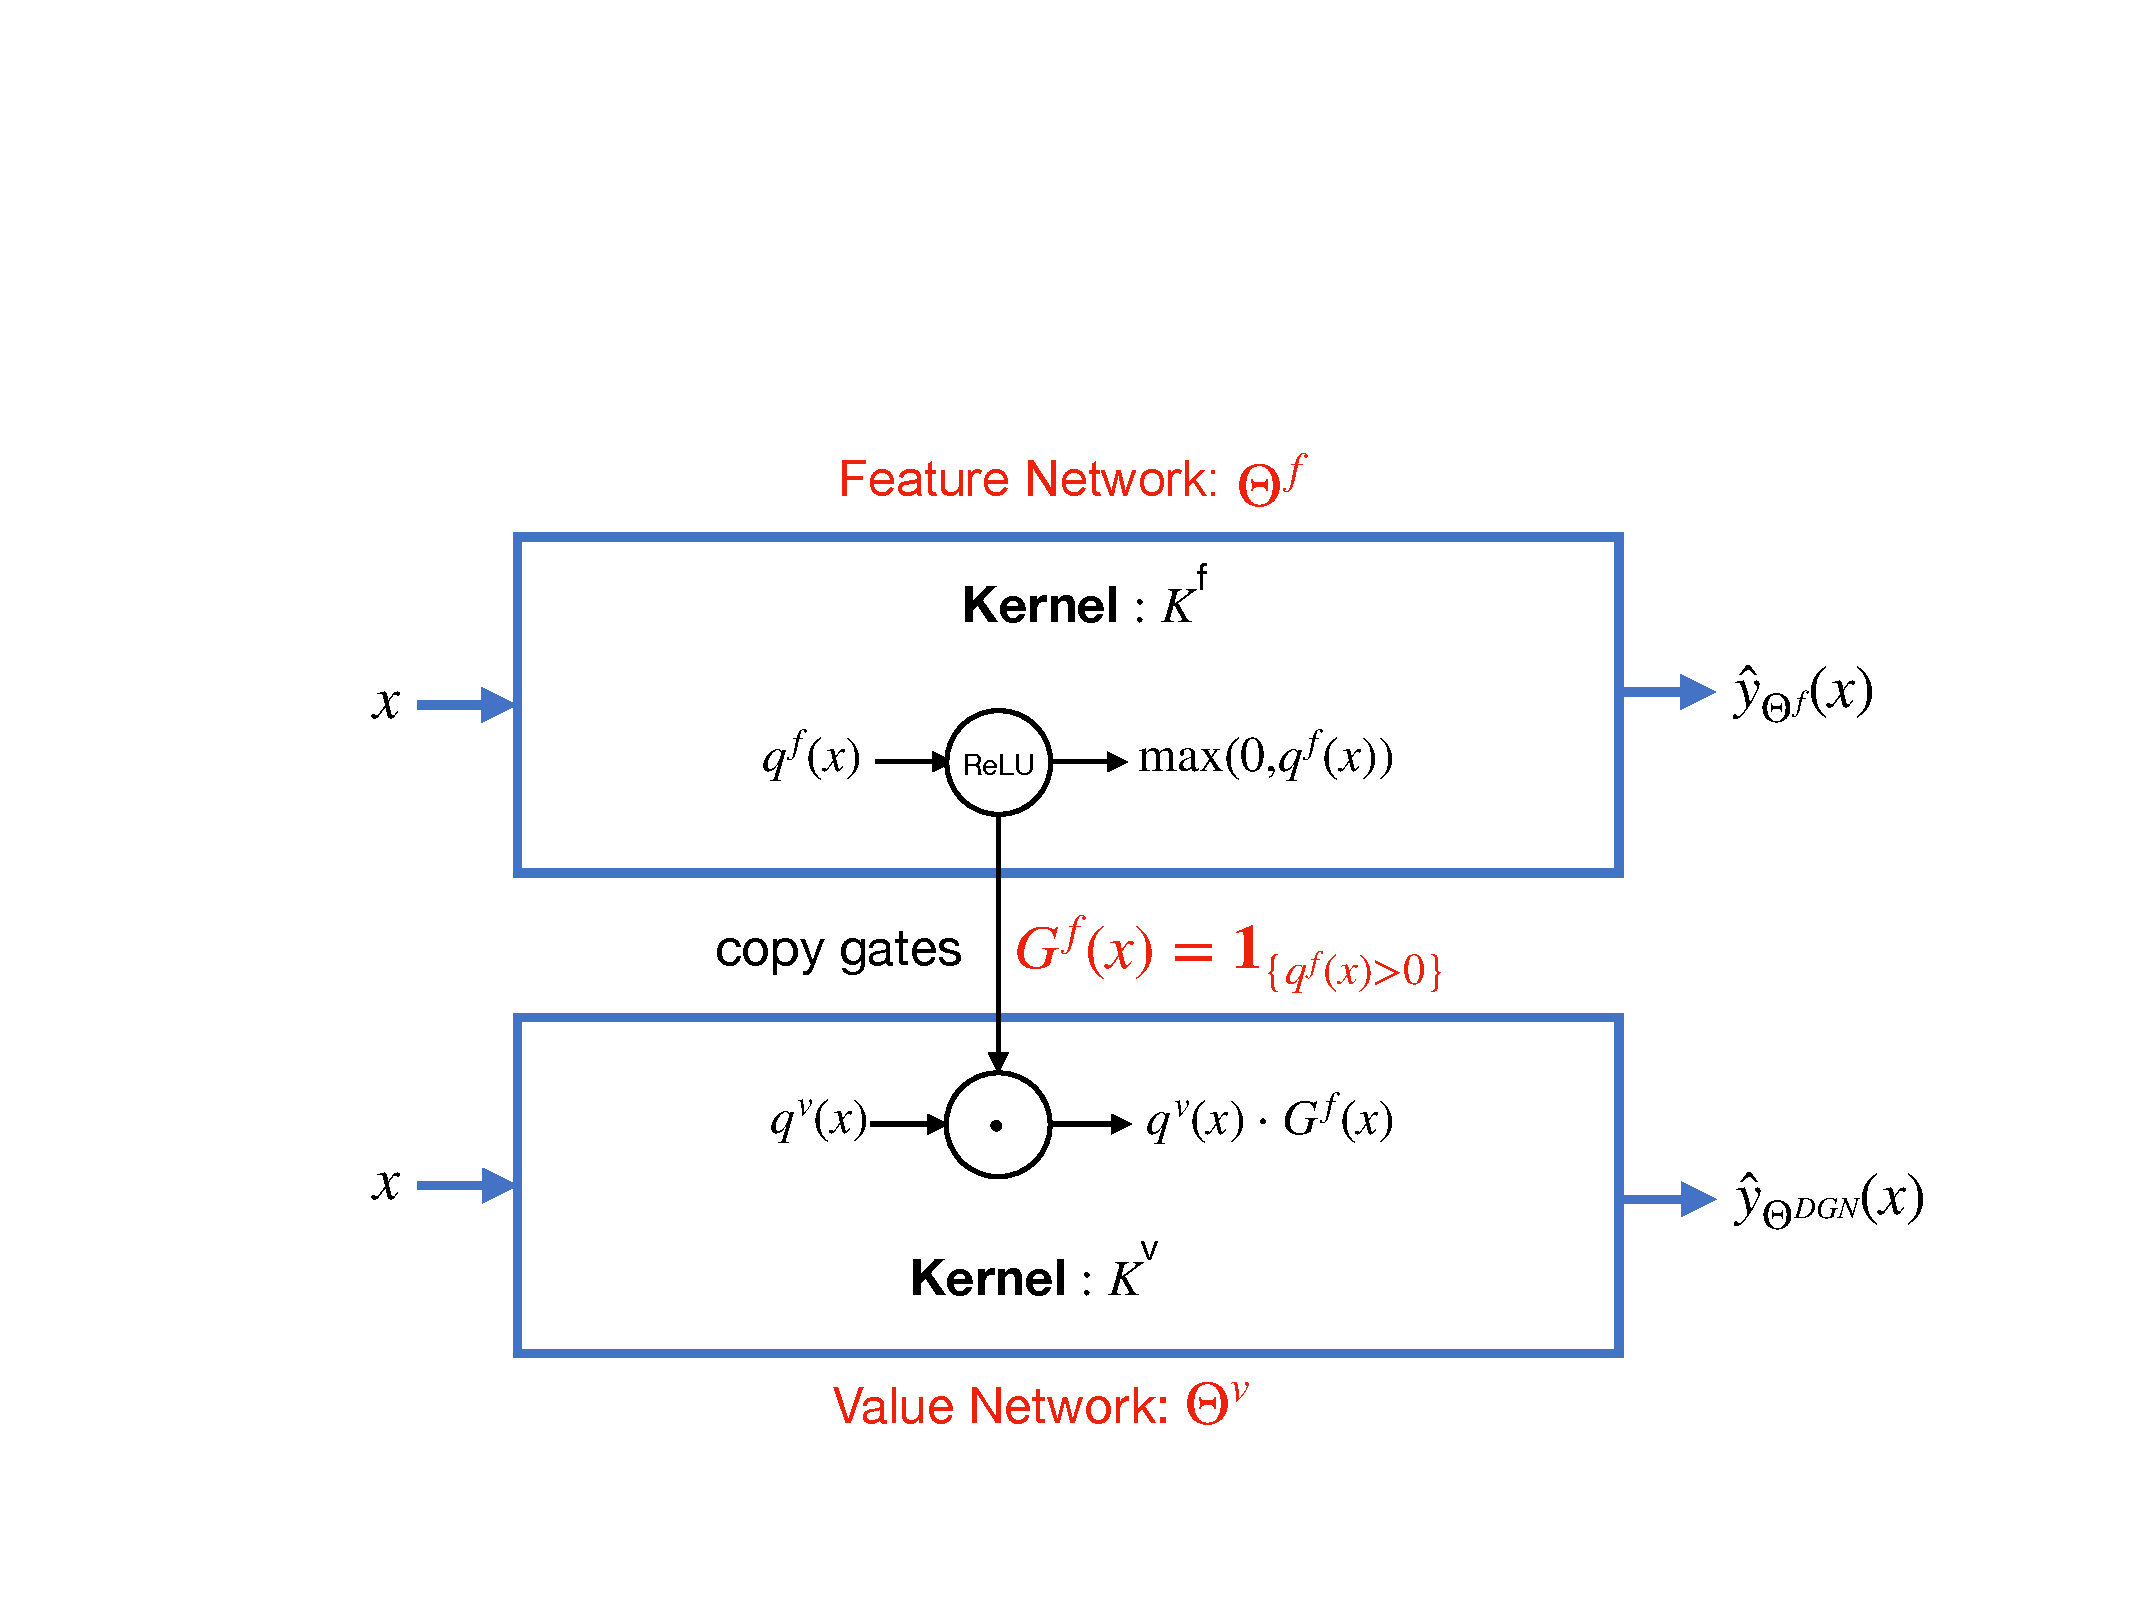
\includegraphics[scale=0.3]{figs/dgn.pdf}
\end{center}
\end{figure}
The DGN has two networks namely the \emph{feature network} parameterised by $\Tf\in\R^{d^{\text{f}}_{\text{net}}}$ which holds the NPFs (i.e., the gating information) and a \emph{value network} parameterised by $\Tv\in\R^{d^{\text{v}}_{\text{net}}}$ which holds the NPV.  The combined parameterisation is denoted by $\Theta^{\text{DGN}}=(\Tf,\Tv)\in \R^{d^{\text{f}}_{\text{net}}+d^{\text{v}}_{\text{net}}}$.  Thus the learning problem in the DGN is $\hat{y}_{\Tdgn}(x)=\ip{\phi_{x,\Tf},v_{\Tv}}$. 
% \subsection{Background: Deep Gated Networks}\label{sec:decoupled}
\begin{comment}
\begin{tabular}{lll}
Feature Network (FN) 	&:&	$\Tf\in\R^{\dfnet}$; provides the gates/masks i.e., the NPFs.\\
Value Network (VN)		&:&	$\Tv\in\R^{\dvnet}$; uses the gates/masks of FN to output $\hat{y}_{\Tdgn}(x)$.\\
Learning Problem &:& $\hat{y}_{\Tdgn}(x)=\ip{\phi_{x,\Tf},v_{\Tv}}$.
\end{tabular}
\end{comment}
\begin{comment}
\begin{wrapfigure}{r}{0.25\textwidth}
  \begin{center}
    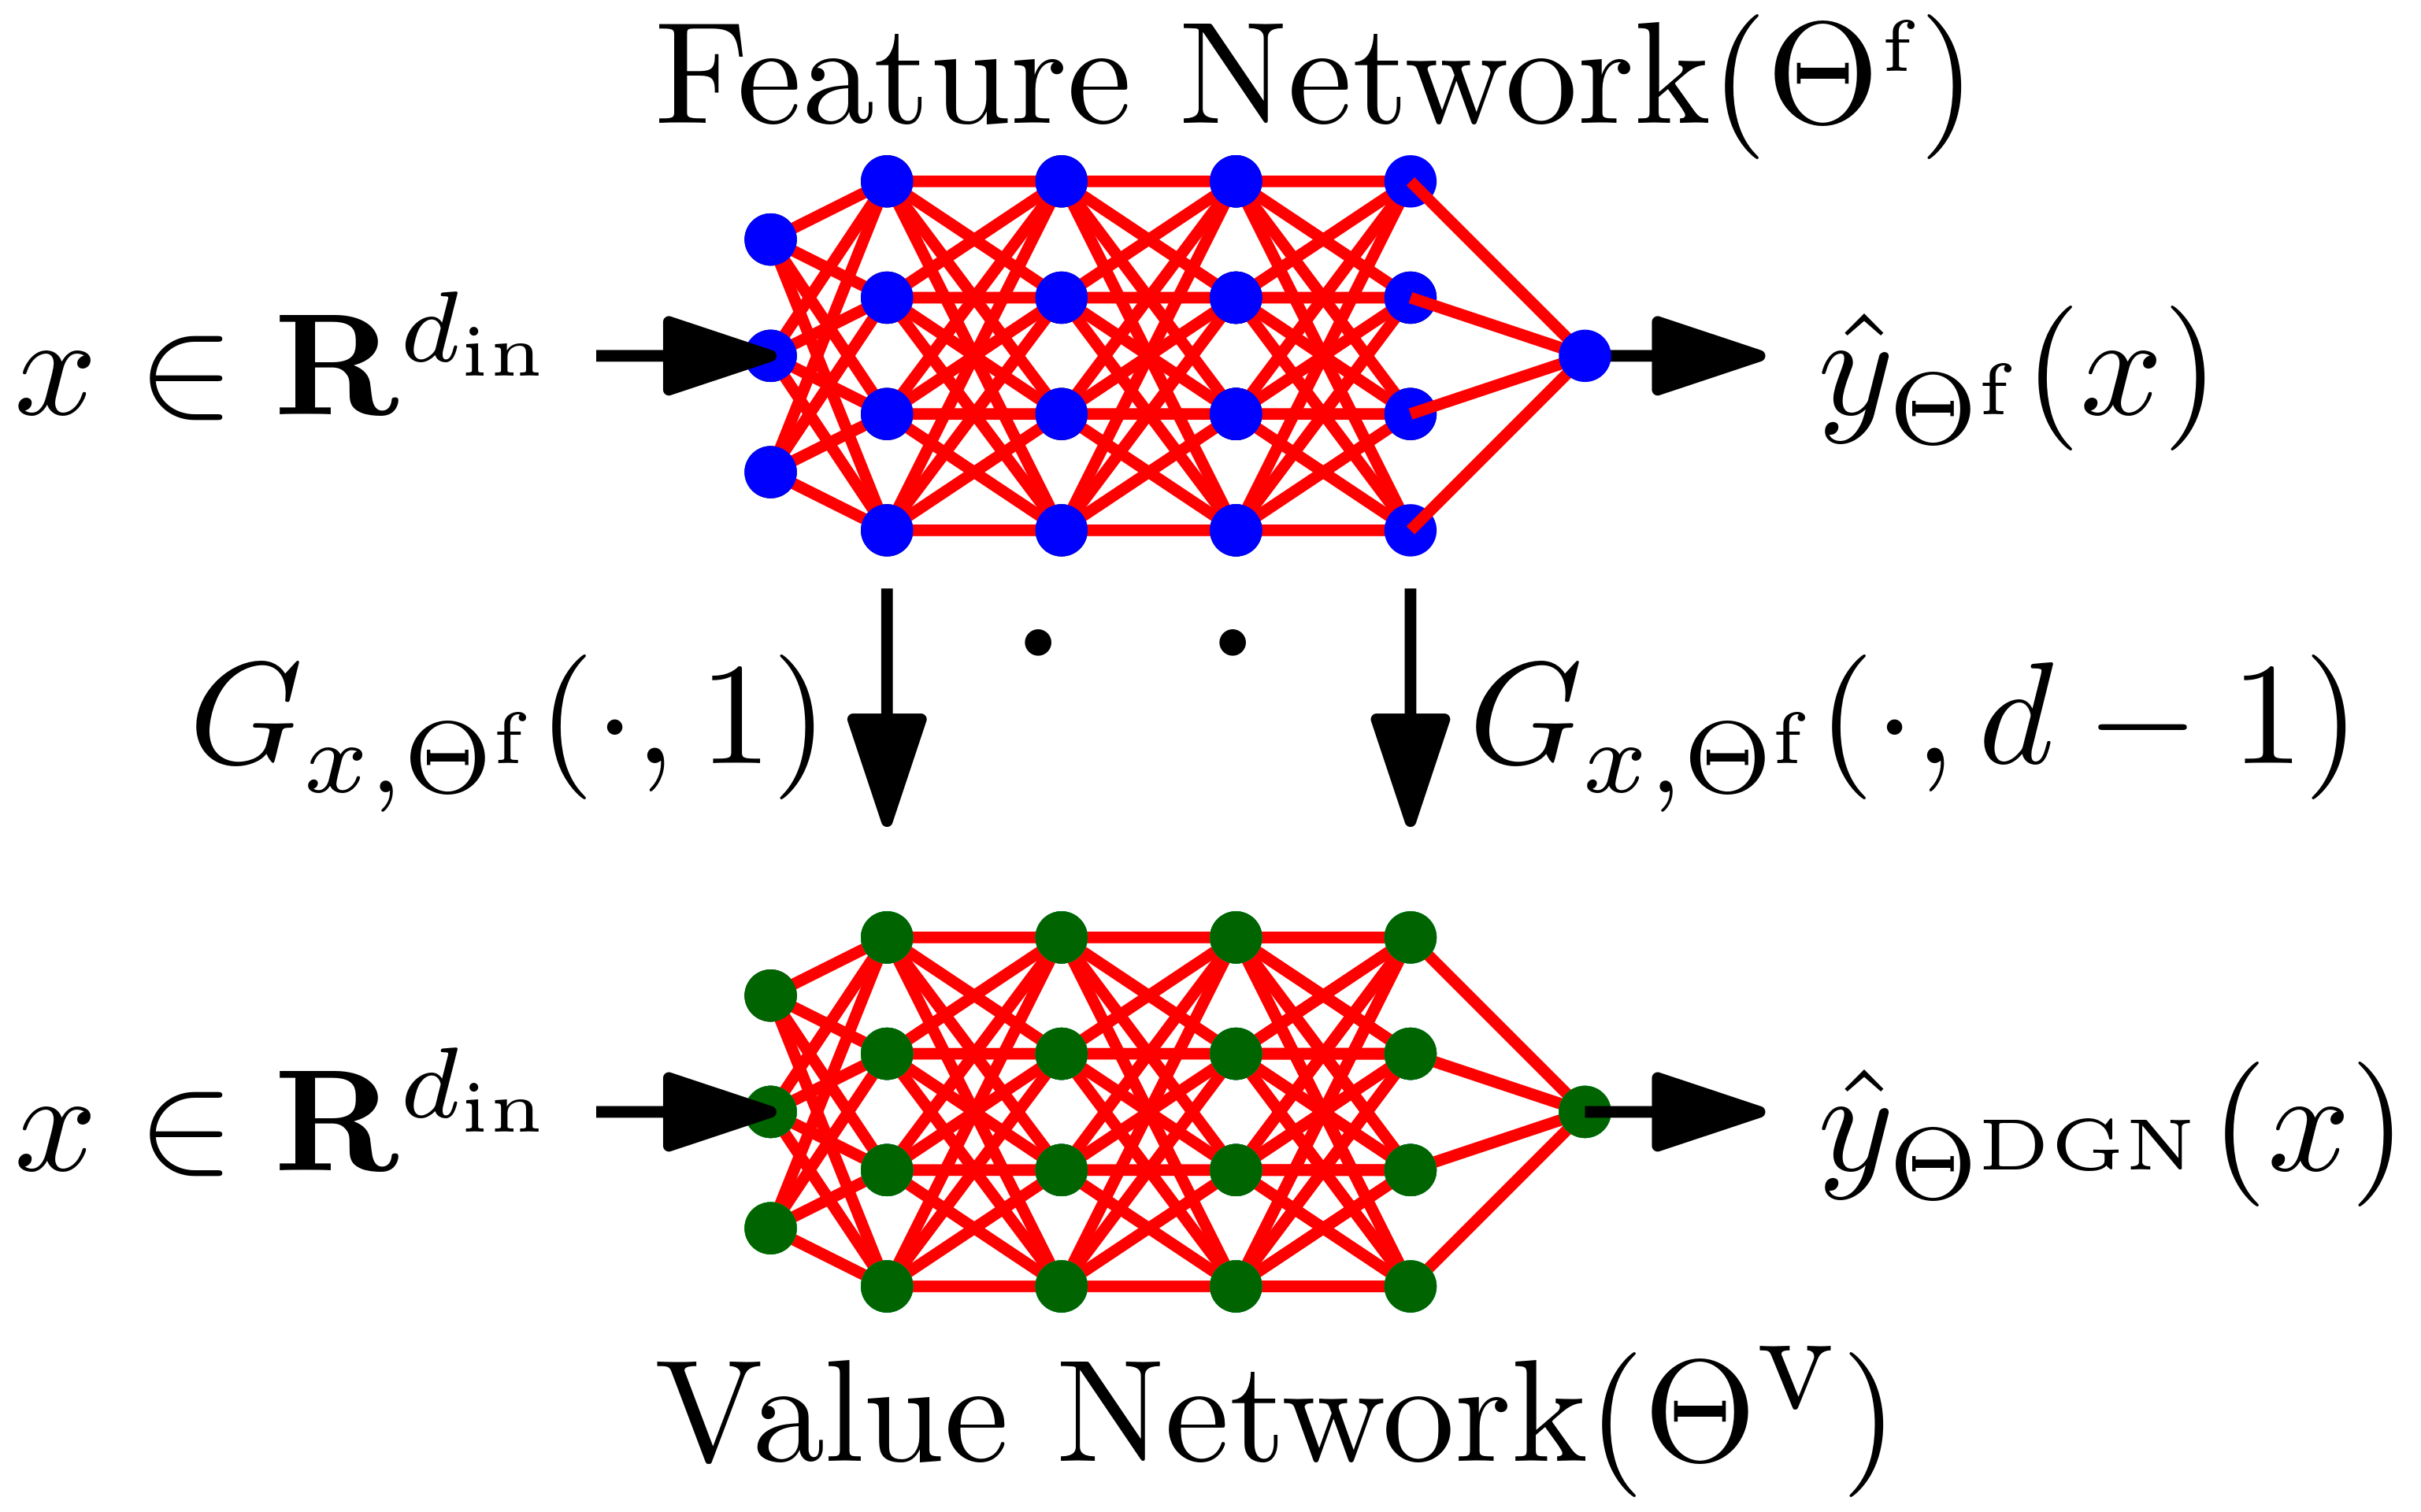
\includegraphics[width=0.25\textwidth]{figs/dgn-small.png}
  \end{center}
\caption{\small{DGN}}
\label{fig:dgn}
\end{wrapfigure}
\end{comment}
\subsection{Regimes of DGN}
% Here the gates/`active sub-networks' are held in the feature network and are then used in the value network.
\begin{definition}\label{rm:regime}The DGN has $\mathbf{4}$ \textbf{regimes} namely \emph{decoupled learning} (DL), \emph{fixed learnt} (FL), \emph{fixed random-dependent initialisation} (FR-DI) and \emph{fixed random-independent initialisation} (FR-II). 
In all the regimes $\hat{y}_{\Tdgn}$ is the output, and $\Tv_0$ is always initialised at random and is \emph{trainable}. However, the regimes differ based on i) trainability of $\Tf$, ii) initialisation $\Tf_0$ as described below.\\
\begin{tabular}{|l|p{6cm}|}\hline
DL               & $\Tf$ is trainable, and $\Tf_0$ and $\Tv_0$ are random and statistically independent,  $\beta>0$.\\\hline
FL               & $\Tf$ is non-trainable, and $\Tf_0$ is pre-trained;  $\Tv_0$ is statistically independent of $\Tf_0$. \\\hline
FR-II            & $\Tf$ is non-trainable, and $\Tf_0$ and $\Tv_0$ are random and statistically independent.\\\hline
FR-DI   &  $\Tf$ is non-trainable, and $\Tf_0=\Tv_0$.\\\hline
\end{tabular}
\end{definition}
The flexibility in a DGN is that  a) $\Tf$ can be trainable/non-trainable and b) $\Tf_0$ can be random or pre-trained using $\hat{y}_{\Tg}$ as the output (\Cref{rm:regime}). By using the DGN setup we can study the role of gates by comparing (a) learnable (DL) vs fixed gates (FL, FR-DI, FR-II), (b) random (FR-DI, FR-II) vs learnt gates (FL) and (c) dependent (FR-DI) vs independent initialisations (FR-II). In the DL regime `soft-ReLU' is chosen to enable gradient flow through the feature network.
%\end{comment}
\begin{comment}\textbf{Flattened Notation:} For a fully connected DNN of width $w$ and depth $d$, there are a total of $\ut=w(d-1)$ hidden units. Let  $q_{x,\Theta}(\iu)$, $G_{x,\Theta}(\iu)$, and $z_{x,\Theta}(\iu)$, where $\iu\in[\ut]$  denote the pre-activation, gating and output values of the $\ut$ hidden unit in the network, whose relationship is given in the left most illustration in \Cref{fig:hunit}.
\FloatBarrier
\begin{table}[h]
\resizebox{\columnwidth}{!}{
\begin{tabular}{|c|c|}\hline
Feature NTK & $\kv_{\Tdgn}(s,s')=\ip{\psiv_{x_s,\Tdgn},\psiv_{x_{s'},\Tdgn}}$, where $\psiv_{x,\Tdgn}=\nabla_{\Tv}\hat{y}_{\Tdgn}(x)\in\R^{\dvnet}$\\\hline
Value NTK & $\kf_{\Tdgn}(s,s')=\ip{\psif_{x_s,\Tdgn},\psif_{x_{s'},\Tdgn}}$, where $\psif_{x,\Tdgn}=\nabla_{\Tf}\hat{y}_{\Tdgn}(x)\in\R^{\dfnet}$\\\hline
\end{tabular}
}
\caption{Definition of NTF and NTKs for DGN used in \Cref{th:main}.}
\label{tb:defks}
\end{table}
\end{comment}
\subsection{NTK = $\text{NTK}^{\text{f}}+ \text{NTK}^\text{v}$}

\begin{proposition}\label{prop:ntks} Let $K_{\Tdgn}$ be the NTK matrix of the DGN, then $K_{\Tdgn}=\kv_{\Tdgn}+\kf_{\Tdgn}$, with
%\FloatBarrier
\begin{table}[h]
\
\begin{tabular}{|c|p{6cm}|}\hline
Overall NTK & $K_{\Tdgn}(s,s')=\ip{\psi_{x_s,\Tdgn},\psi_{x_{s'},\Tdgn}}$, where $\psi_{x,\Tdgn}=\nabla_{\Tdgn}\hat{y}_{\Tdgn}(x)\in\R^{\dnet}$\\\hline
Feature NTK & $\kv_{\Tdgn}(s,s')=\ip{\psiv_{x_s,\Tdgn},\psiv_{x_{s'},\Tdgn}}$, where $\psiv_{x,\Tdgn}=\nabla_{\Tv}\hat{y}_{\Tdgn}(x)\in\R^{\dvnet}$\\\hline
Value NTK & $\kf_{\Tdgn}(s,s')=\ip{\psif_{x_s,\Tdgn},\psif_{x_{s'},\Tdgn}}$, where $\psif_{x,\Tdgn}=\nabla_{\Tf}\hat{y}_{\Tdgn}(x)\in\R^{\dfnet}$\\\hline
\end{tabular}

\end{table}
\end{proposition}
\textbf{Remark:} There are two separate NTKs, each one corresponding to feature and value networks respectively. In the case of fixed regimes, $\kf=0$. 
